\documentclass[10pt]{beamer}

% Configuration {{{
\usepackage[utf8]{inputenc}
\usepackage[T2A]{fontenc} % T1 for English
\usepackage[english, russian]{babel}

\usepackage{mathtools}
\usepackage{graphicx}
\usepackage{tikz}
\usepackage[multidot]{grffile}
\usepackage[labelsep=period]{caption}
\usepackage{multirow}

\setbeamertemplate{caption}[numbered]
\setbeamertemplate{navigation symbols}{}
\usefonttheme[onlymath]{serif}
\usepackage{DejaVuSansCondensed} % helvet for English
\usetheme{Madrid}

\linespread{1.2}
% }}}

% Title and other {{{
\title[Measurements of charmed baryons]{
  Measurements of the properties of $\Lambda_c(2595)$, 
  $\Lambda_c(2625)$, $\Sigma_c(2455)$, $\Sigma_c(2520)$ baryons
  by CDF
  -- contents analysis
}
\author[Kerim Guseynov]{
  Kerim Guseynov \\[2ex] Based on \texttt{arXiv:1105.5995}
}
\institute[MSU]{
  Faculty of Physics \\ Moscow State University
}
\date{Nov 11, 2022}
%}}}

\begin{document}

\frame[plain]{\titlepage}

\begin{frame}[label=intro]%{{{
  \frametitle{Introduction \& motivation}

  \centering
  \parbox{.6\textwidth}{
    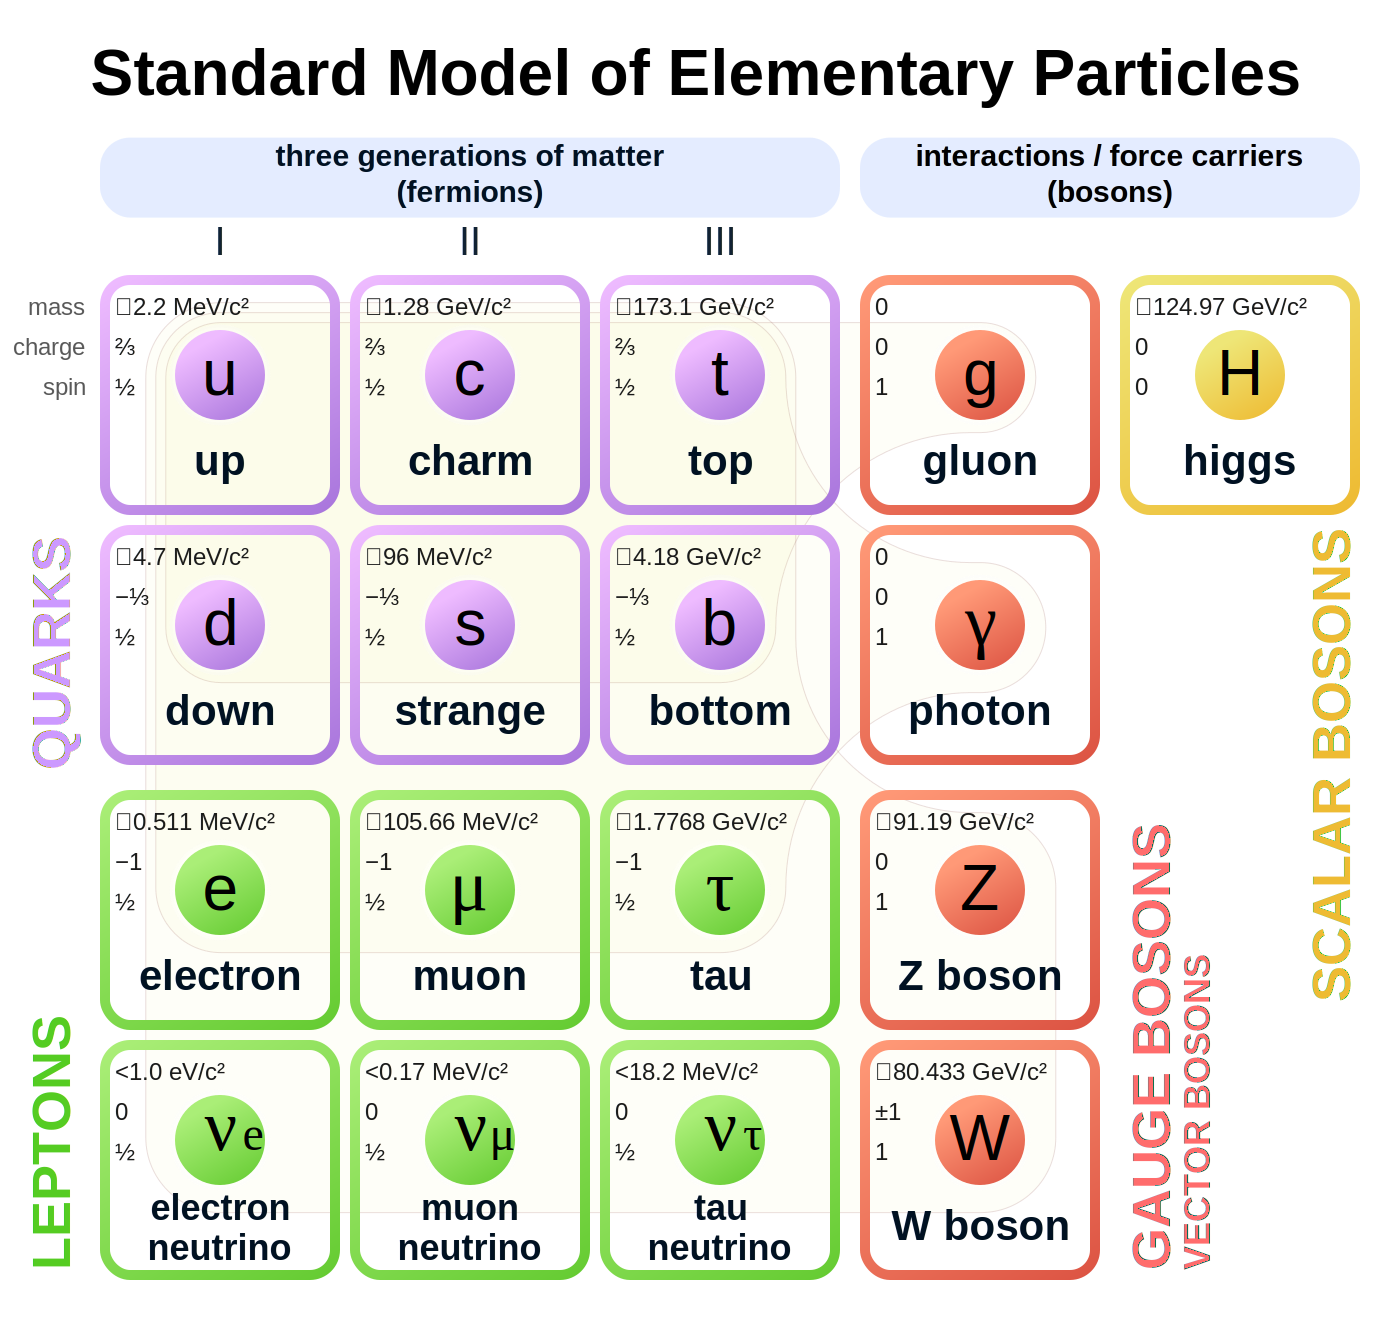
\includegraphics[width=\linewidth]{figures/001/stdmod}
  } \hspace*{2ex} \parbox{.35\textwidth}{
    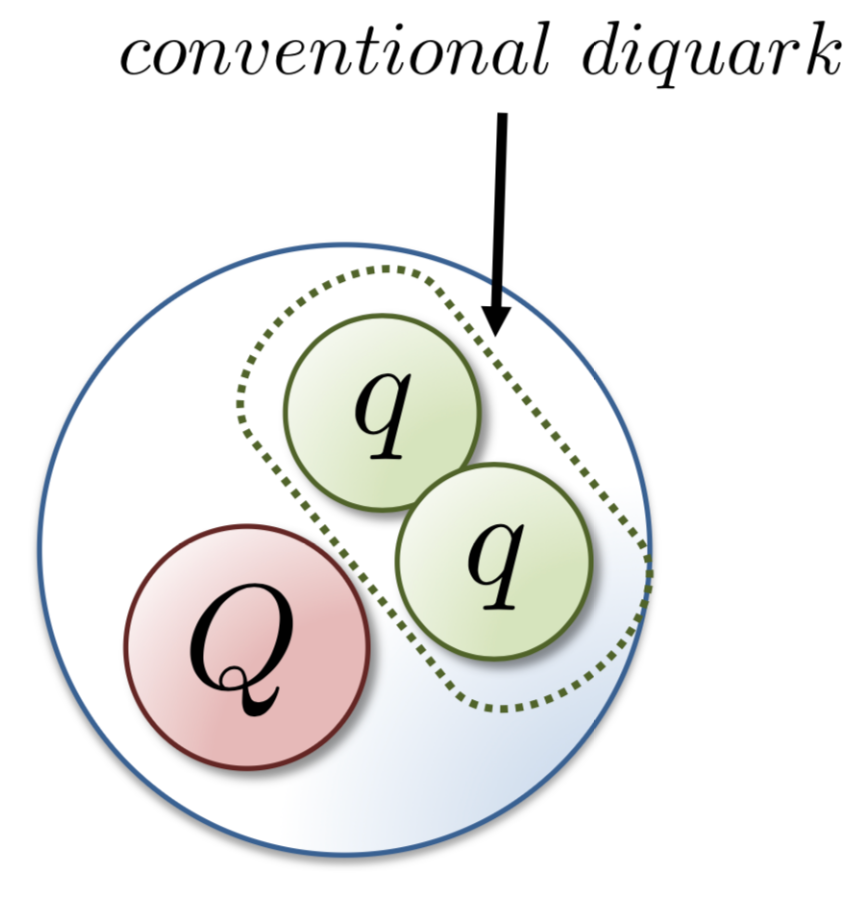
\includegraphics[width=\linewidth]{figures/001/heavy-baryon-Qqq}
    \vskip 1ex
    \begin{tabular}{cc}
      $\Sigma_c(2455)^{++}$ & $\Sigma_c(2455)^{0}$ \\
      $\Sigma_c(2520)^{++}$ & $\Sigma_c(2520)^{0}$ \\
      $\Lambda_c(2595)^{+}$ & $\Lambda_c(2625)^{+}$ \\
    \end{tabular}
  }

  % heavy (with c and b) provide unique possibilities for studying QCD.
  % Large alpha_s -> no perturbative 
  %
  % longer useless text {{{
  % Hadrons containing a heavy $c$ or $b$ quark, called heavy hadrons, 
  % provide unique possibilities for studying and testing QCD, the 
  % theory of strong interactions. Because of the large strong coupling 
  % constant $\alpha_s$ at smaller momenta transfers, perturbative QCD 
  % is not applicable to theoretical studies of any hadrons, including 
  % heavy ones. At the same time, the presence of a heavy quark gives at 
  % least some starting point and allows for vague analogies with  
  % well-known and well-studied electromagnetic systems, which can then 
  % be modified and reinforced.
  %
  % Thus many different approaches were developed for the description of 
  % heavy hadrons, including, for example, heavy quark effective theory, 
  % relativistic potential models, lattice QCD, QCD sum rules.
  %
  % The basic structure of a heavy hadron can in some sense be viewed as 
  % a hydrogen atom of QCD. Mesons are made up of a heavy quark and 
  % a light quark and bear a marginally better resemblance to a nucleus 
  % with an electron orbiting around it compared to baryons, which 
  % consist of a heavy quark and a light diquark. But this resemblance 
  % is so weak in the first place that the difference is negligible in 
  % the end.
  %
  % As a result, a multitude of theoretical predictions were made for 
  % the numerous heavy baryons and their resonant states. This article 
  % concerns with six resonant states of charmed baryons Lc and Sc.
  %}}}
\end{frame}%}}}

\begin{frame}[label=prev-exp]%{{{
  \frametitle{World average values at the time of this analysis}
  \centering
  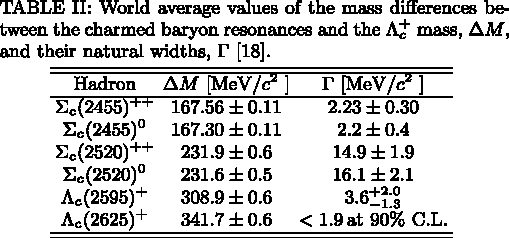
\includegraphics[width=.8\textwidth]{figures/001/table-ii}

  % At the time of this analysis, the world average values of masses and 
  % widths of the studied resonances had already been measured by 
  % several collaborations. But the data samples had never been as large 
  % and precise as the ones used for this analysis. It is especially 
  % true for Lc resonances.
\end{frame}%}}}

\begin{frame}[label=events]%{{{
  \frametitle{Experimental data selection}

  \begin{itemize}
    \item Based on data from CDF II detector at Tevatron.
      \\ Collected from 2002 to 2009: $5.2$ fb$^{-1}$ of integrated 
      luminosity.
    \item Tracking system,
      \\ Momentum measurement,
      \\ Energy measurement,
      \\ Time-of-flight sensor.
      \\ Combined, they also provide particle identification.
    \item Event selection in several steps using neural networks at each 
      one.
      \begin{itemize}
        \item Selection of $\Lambda_c^+$ (ground state) candidates in 
          $pK^-\pi^+$ spectrum.
        \item Selection of $\Sigma_c(2455)$ candidates in 
          $\Lambda_c^+\pi^\pm$ mass spectra.
        \item Selection of $\Lambda_c(2625)^+$ candidates in 
          $\Lambda_c^+\pi^+\pi^-$ spectrum.
      \end{itemize}
  \end{itemize}
\end{frame}%}}}

\begin{frame}[label=selection-Lc]%{{{
  \frametitle{Selection of $\Lambda_c^+$ candidates}
  \centering
  \parbox{.48\textwidth}{
    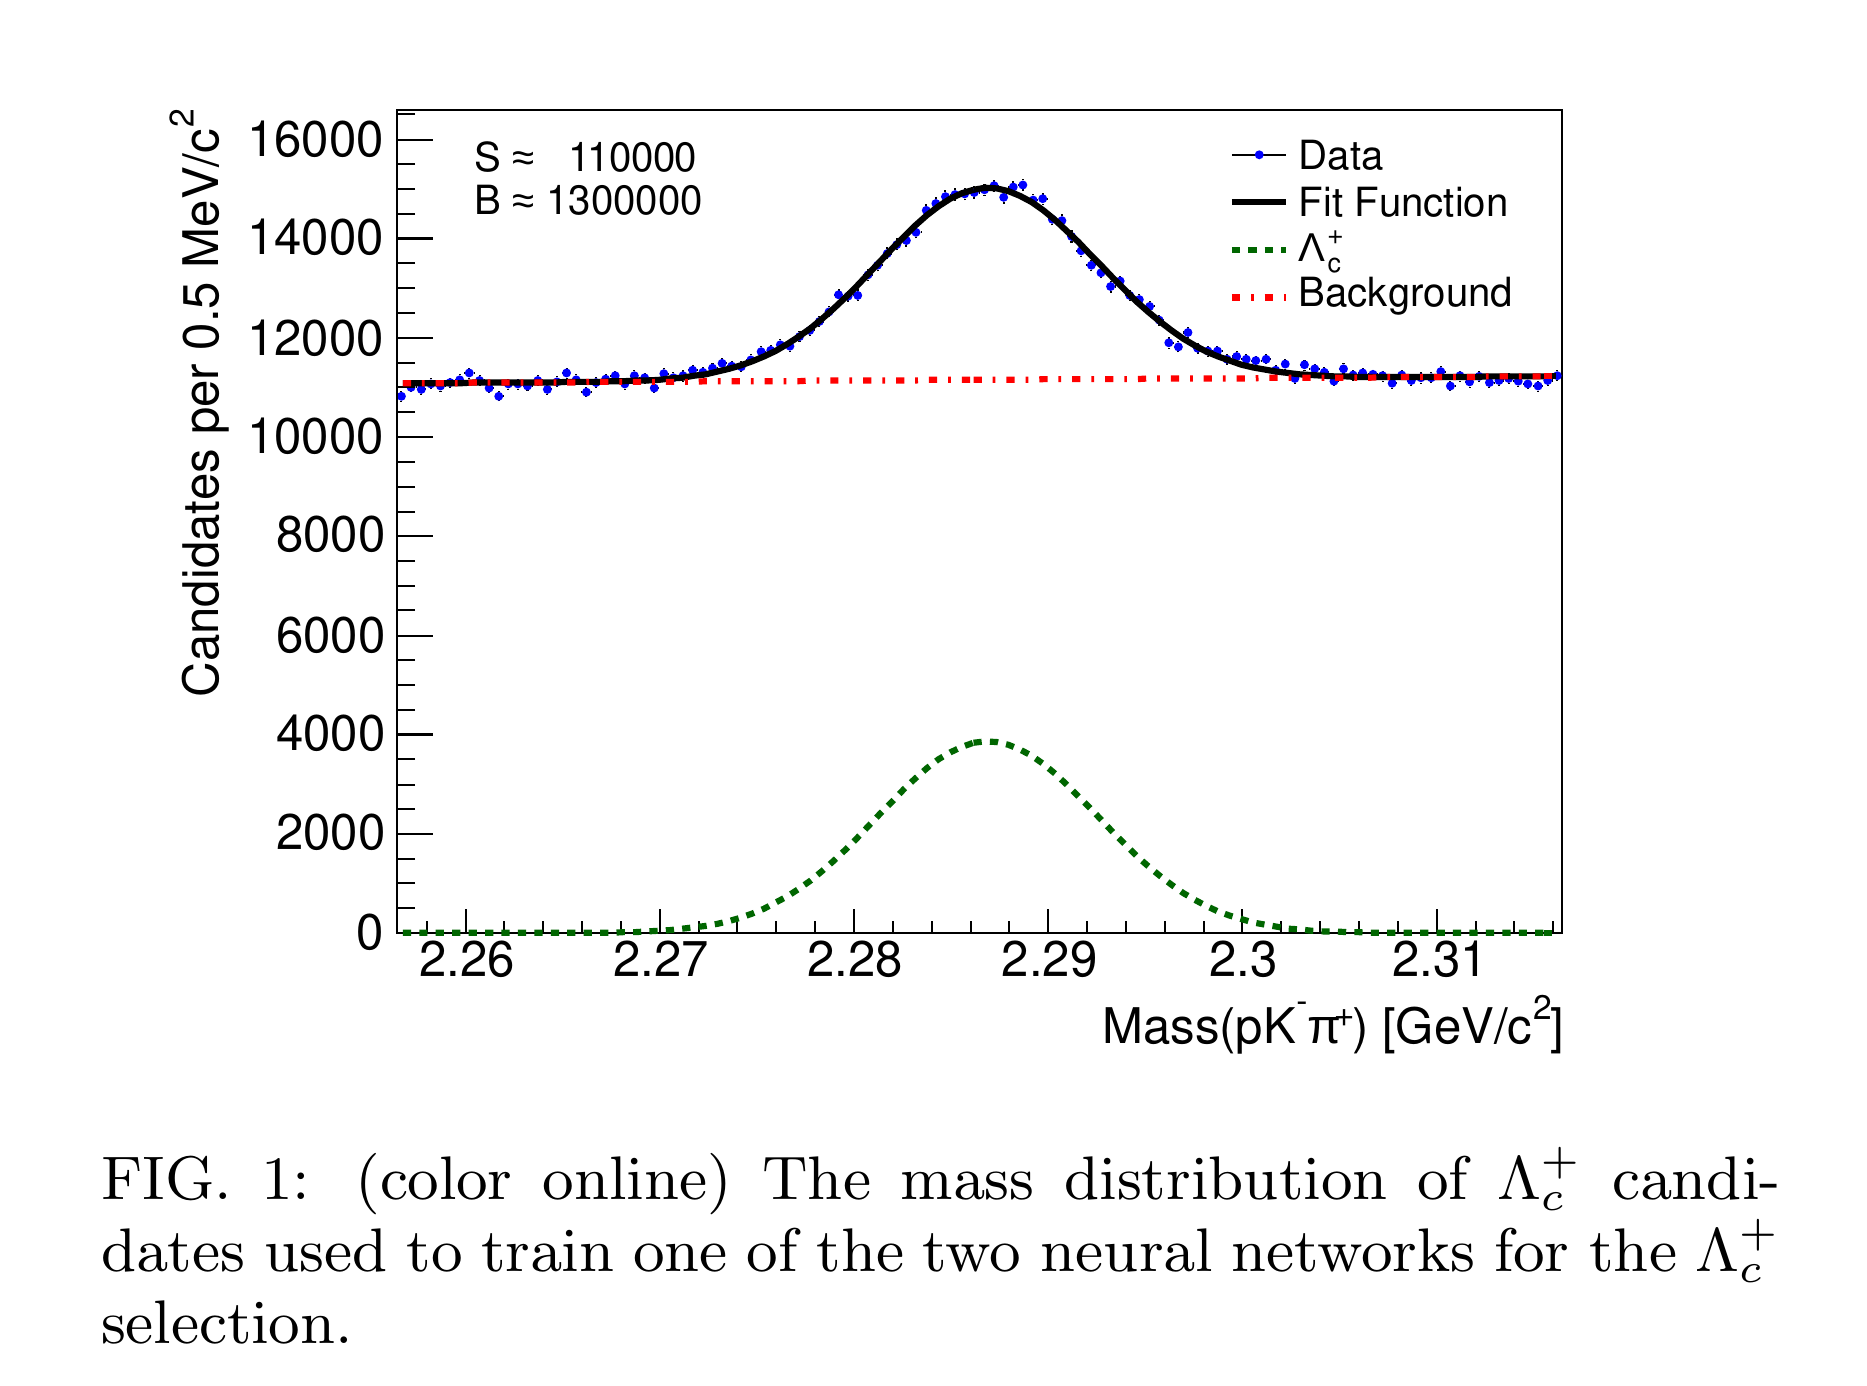
\includegraphics[width=.48\textwidth]{figures/001/initial-Lc}
  } \parbox{.48\textwidth}{
    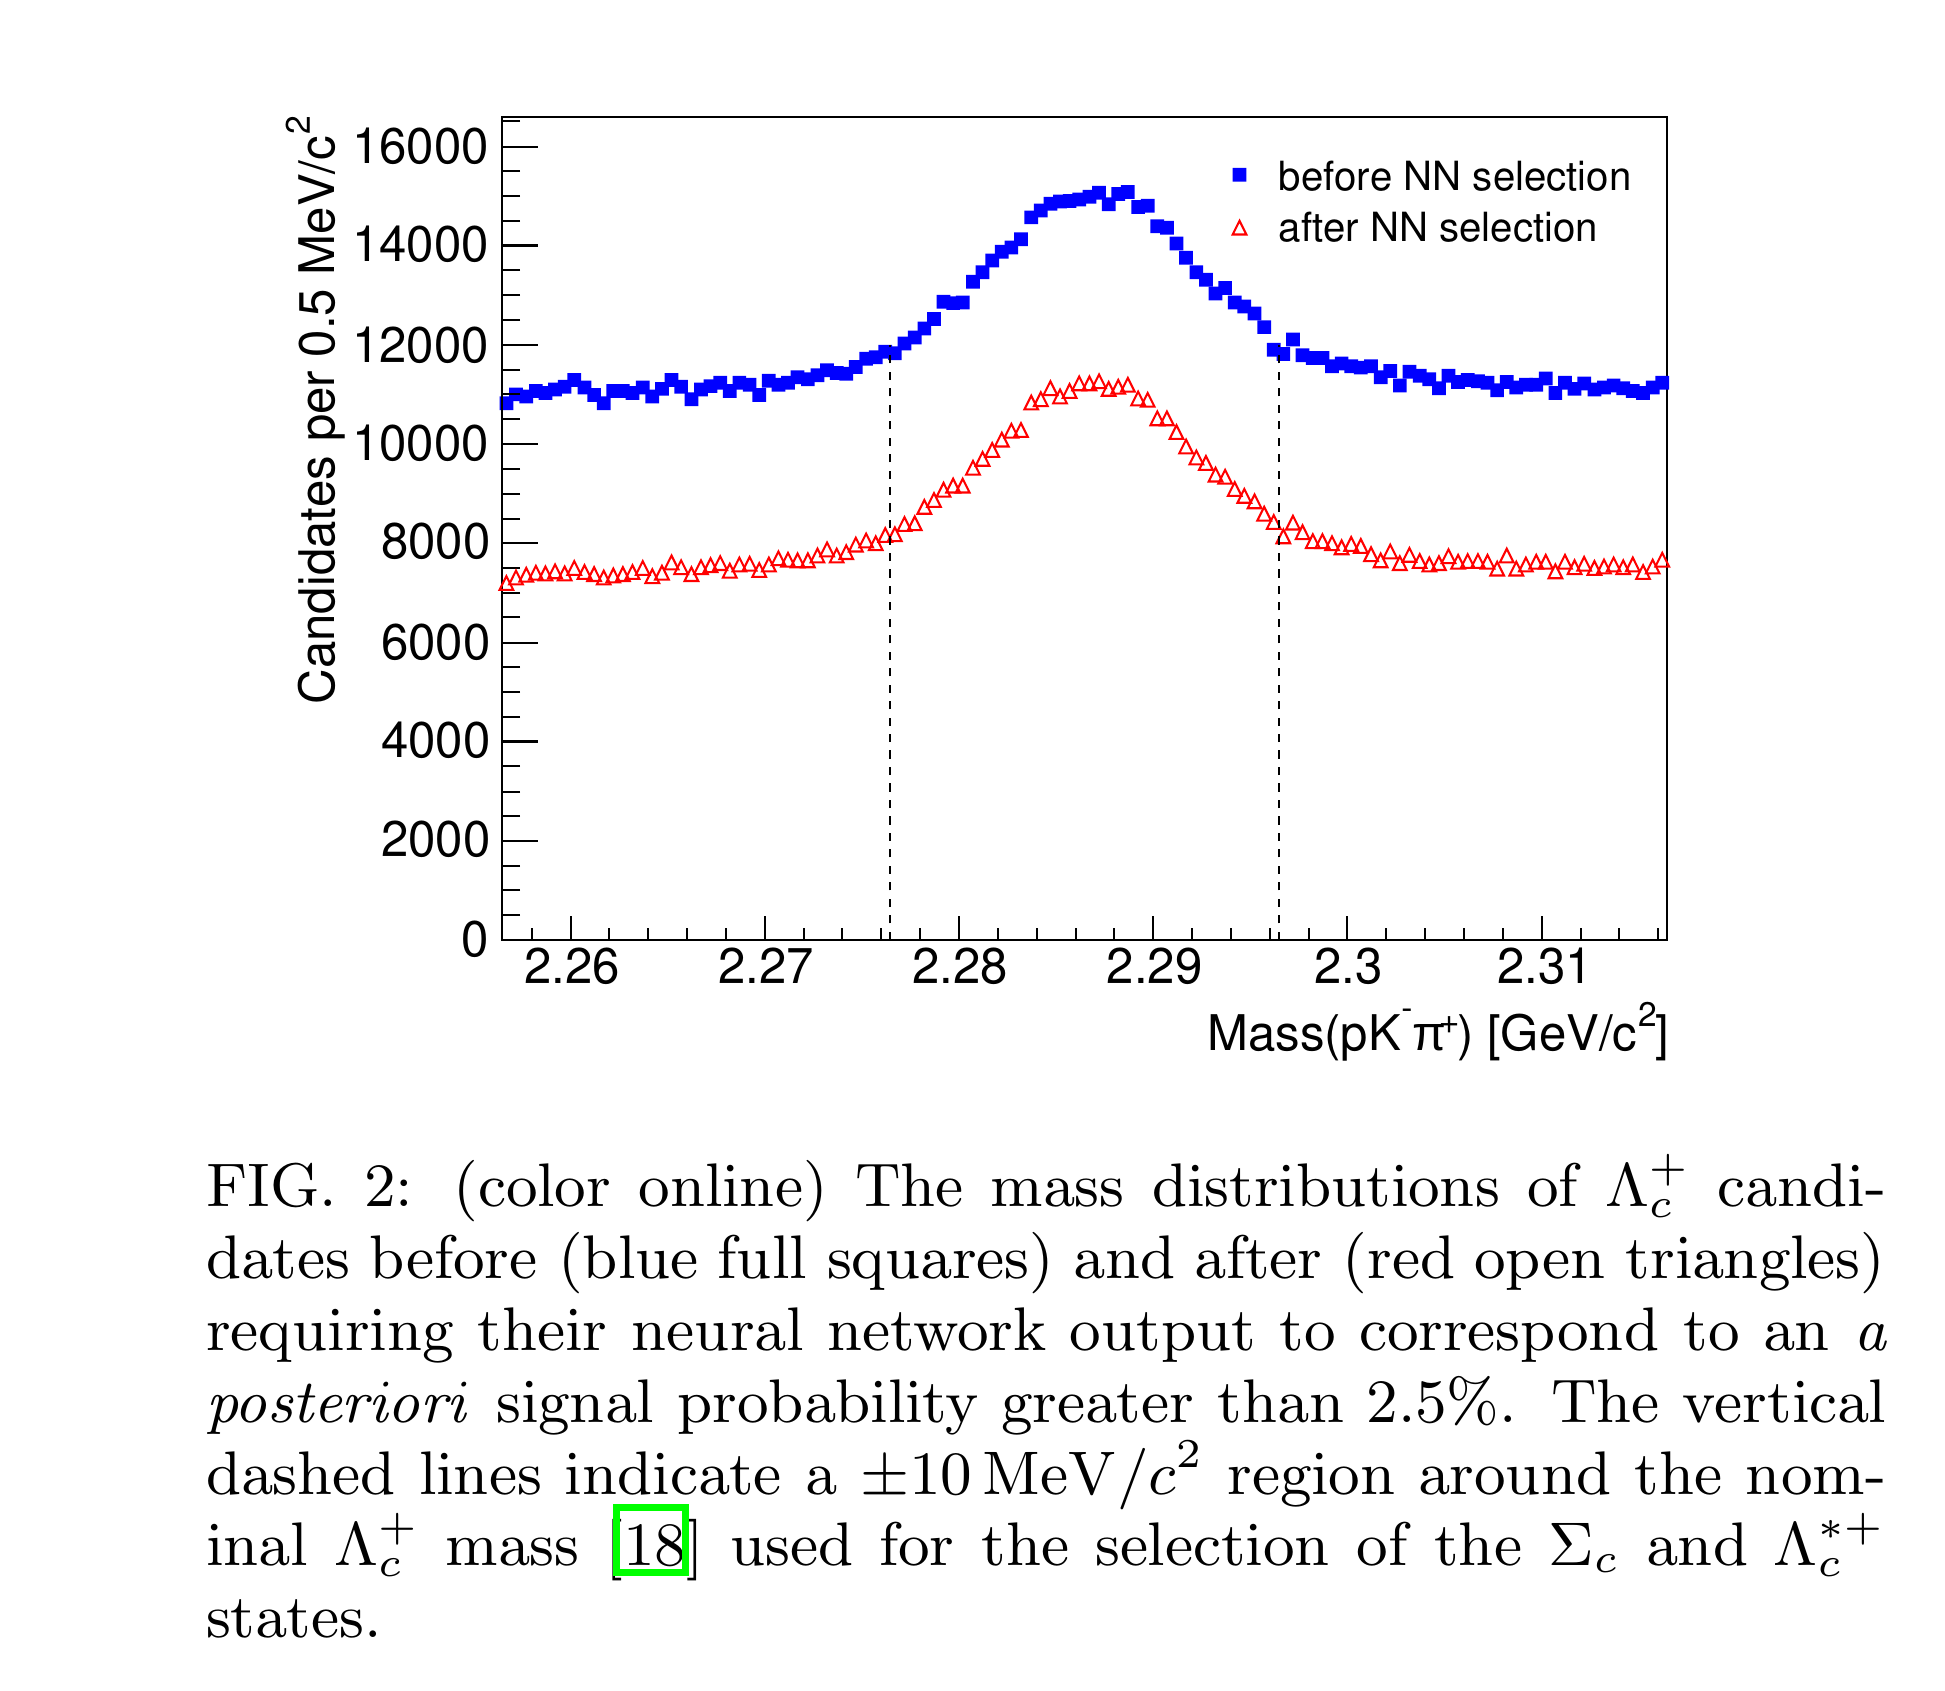
\includegraphics[width=.48\textwidth]{figures/001/after-Lc}
  }

  % The selection of Lc is performed in two stages. First, some loose 
  % selection criteria are applied to suppress the most obvious 
  % background. And then a neural network is trained to figure out 
  % characteristics of signal events and distinguish it from the 
  % combinatorial background. The training procedure is performed 
  % entirely based on experimental data. So, to prevent overtraining and 
  % biases, the full data set is randomly split in two halves, and two 
  % separate neural networks are trained on one half and then applied to 
  % the other. The result of such selection is shown on the right in 
  % red.
\end{frame}%}}}

\begin{frame}[label=selection-Sc*]%{{{
  \frametitle{Event selection in $\Lambda_c^+\pi^\pm$ spectra}
  \centering
  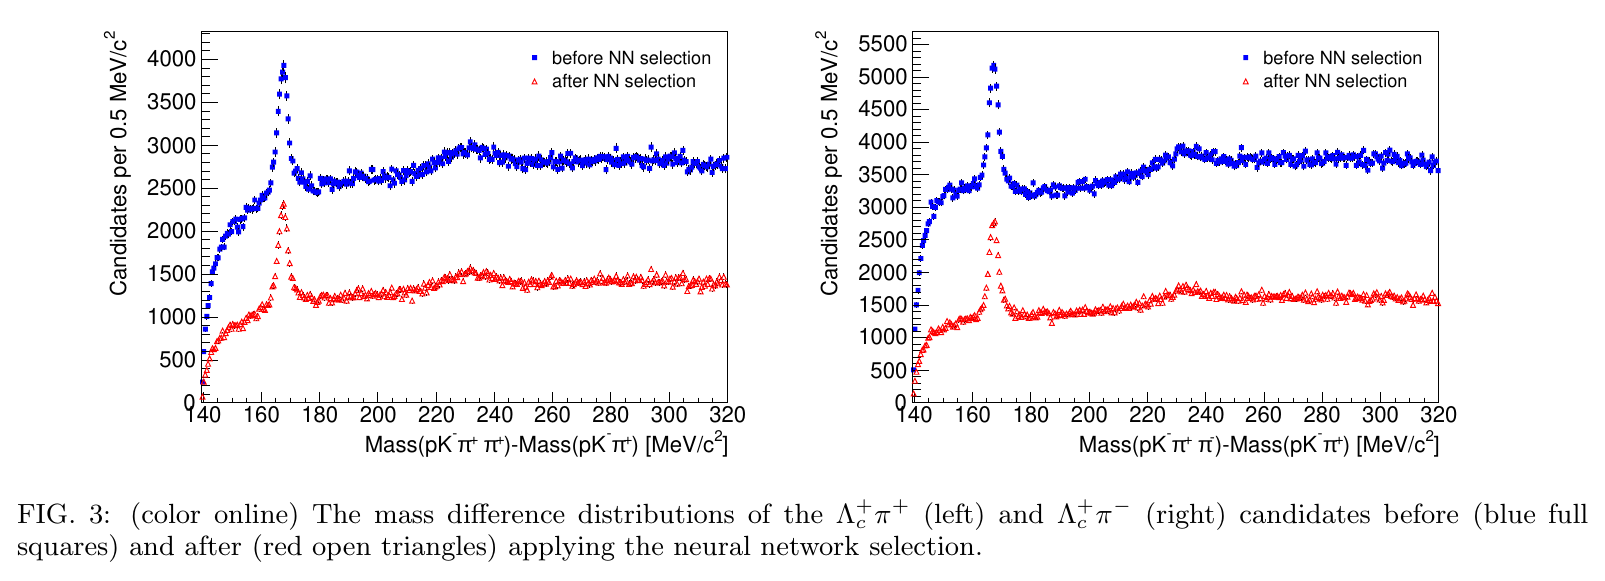
\includegraphics[width=\textwidth]{figures/001/selection-Scstar}

  % A similar two-stage process with two subsets of data is then 
  % repeated for Lcpi spectra to improve signal quality. Only the most 
  % prominent, the first, peak is used for selection, but the result is 
  % used to measure both resonances anyway.
\end{frame}%}}}

\begin{frame}[label=selection-Lc*]%{{{
  \frametitle{Event selection in $\Lambda_c^+\pi^+\pi^-$ spectrum}
  \centering
  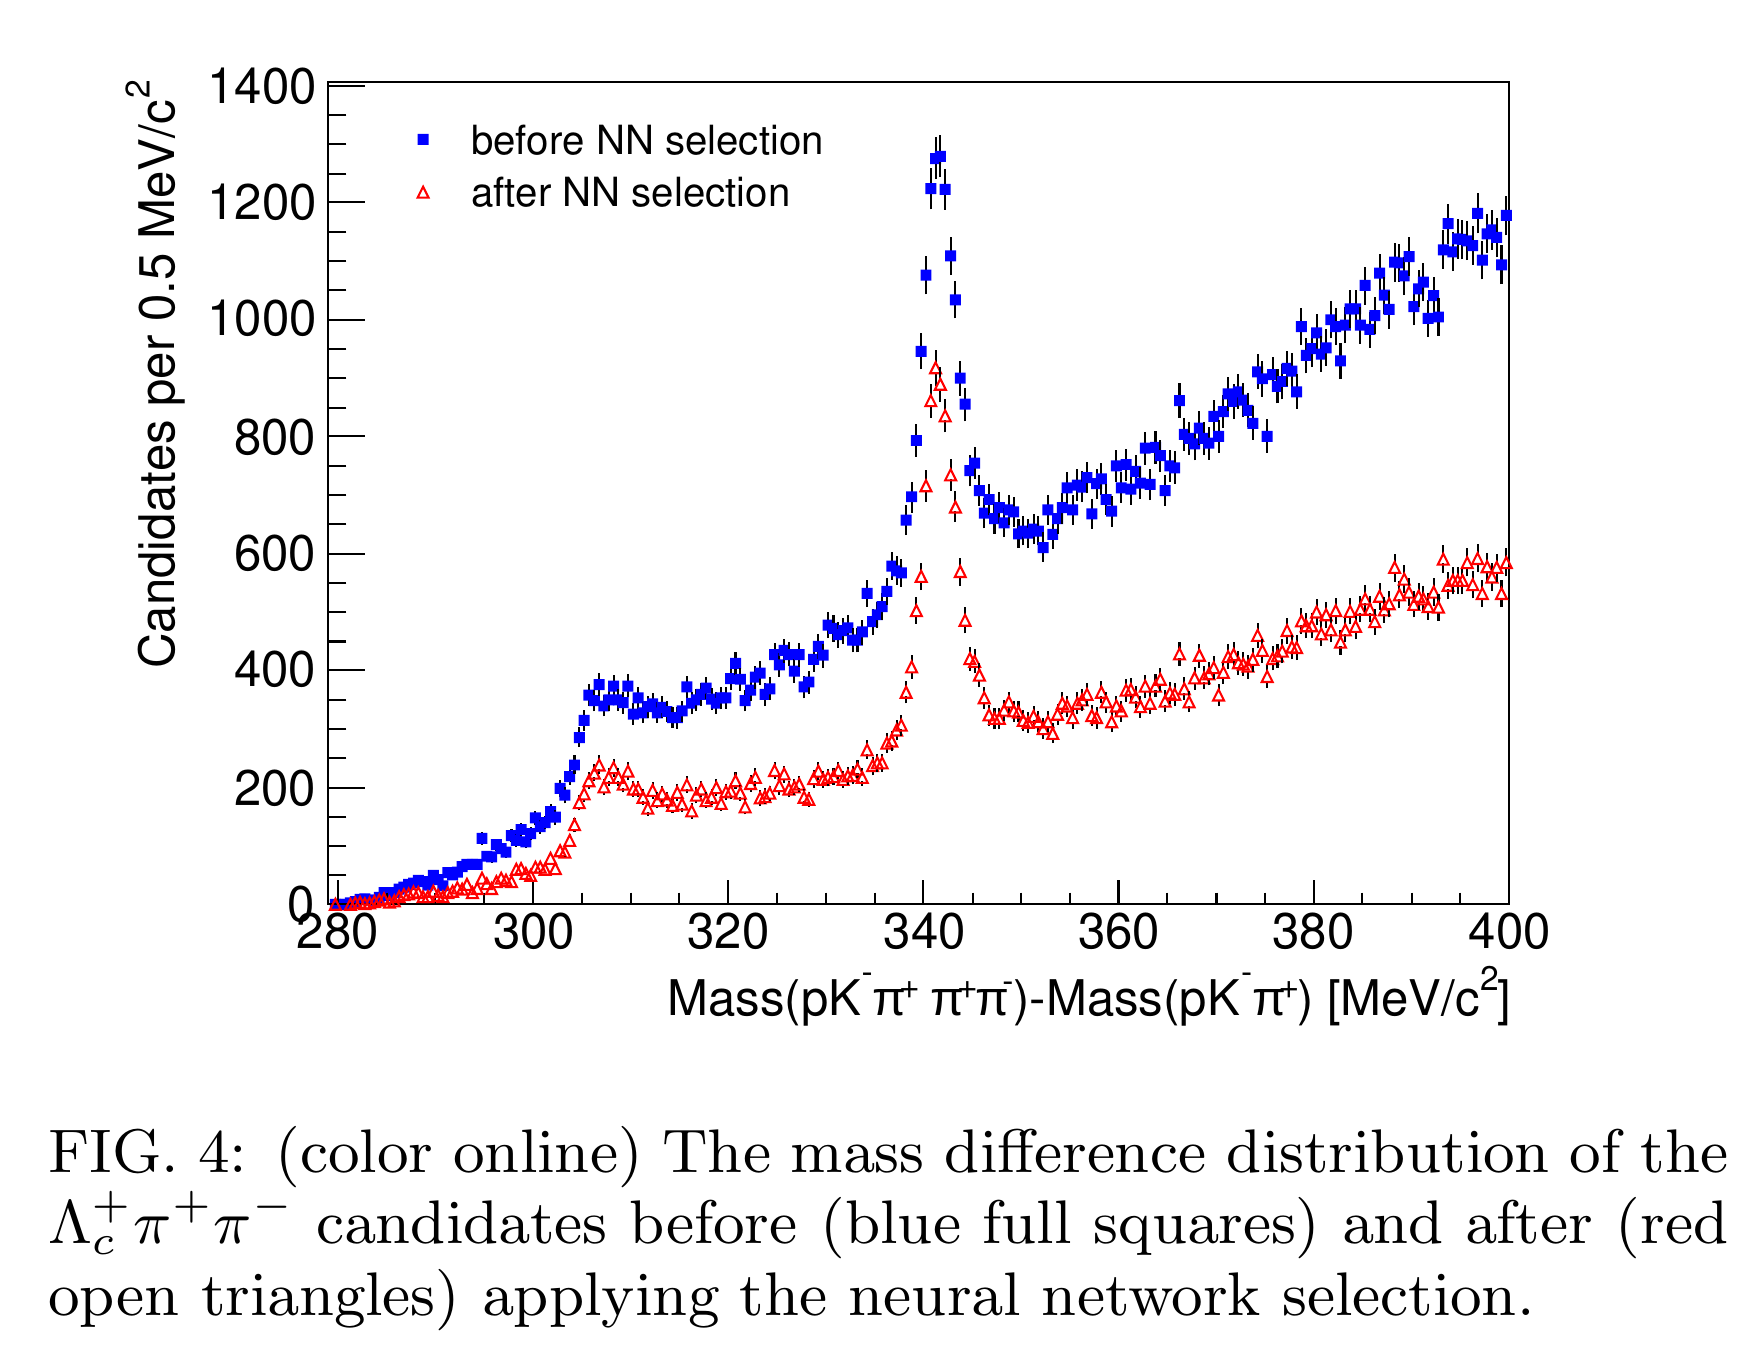
\includegraphics[width=.7\textwidth]{figures/001/selection-Lcstar}

  % And another similar procedure is applied to Lcpipi spectrum for 
  % event selection. Again, only the most prominent peak, the second in 
  % this case, was used in training.
\end{frame}%}}}

\begin{frame}[label=fit-Sc*]%{{{
  \frametitle{Models and approximation of $\Lambda_c^+\pi^\pm$ spectra}
  \centering
  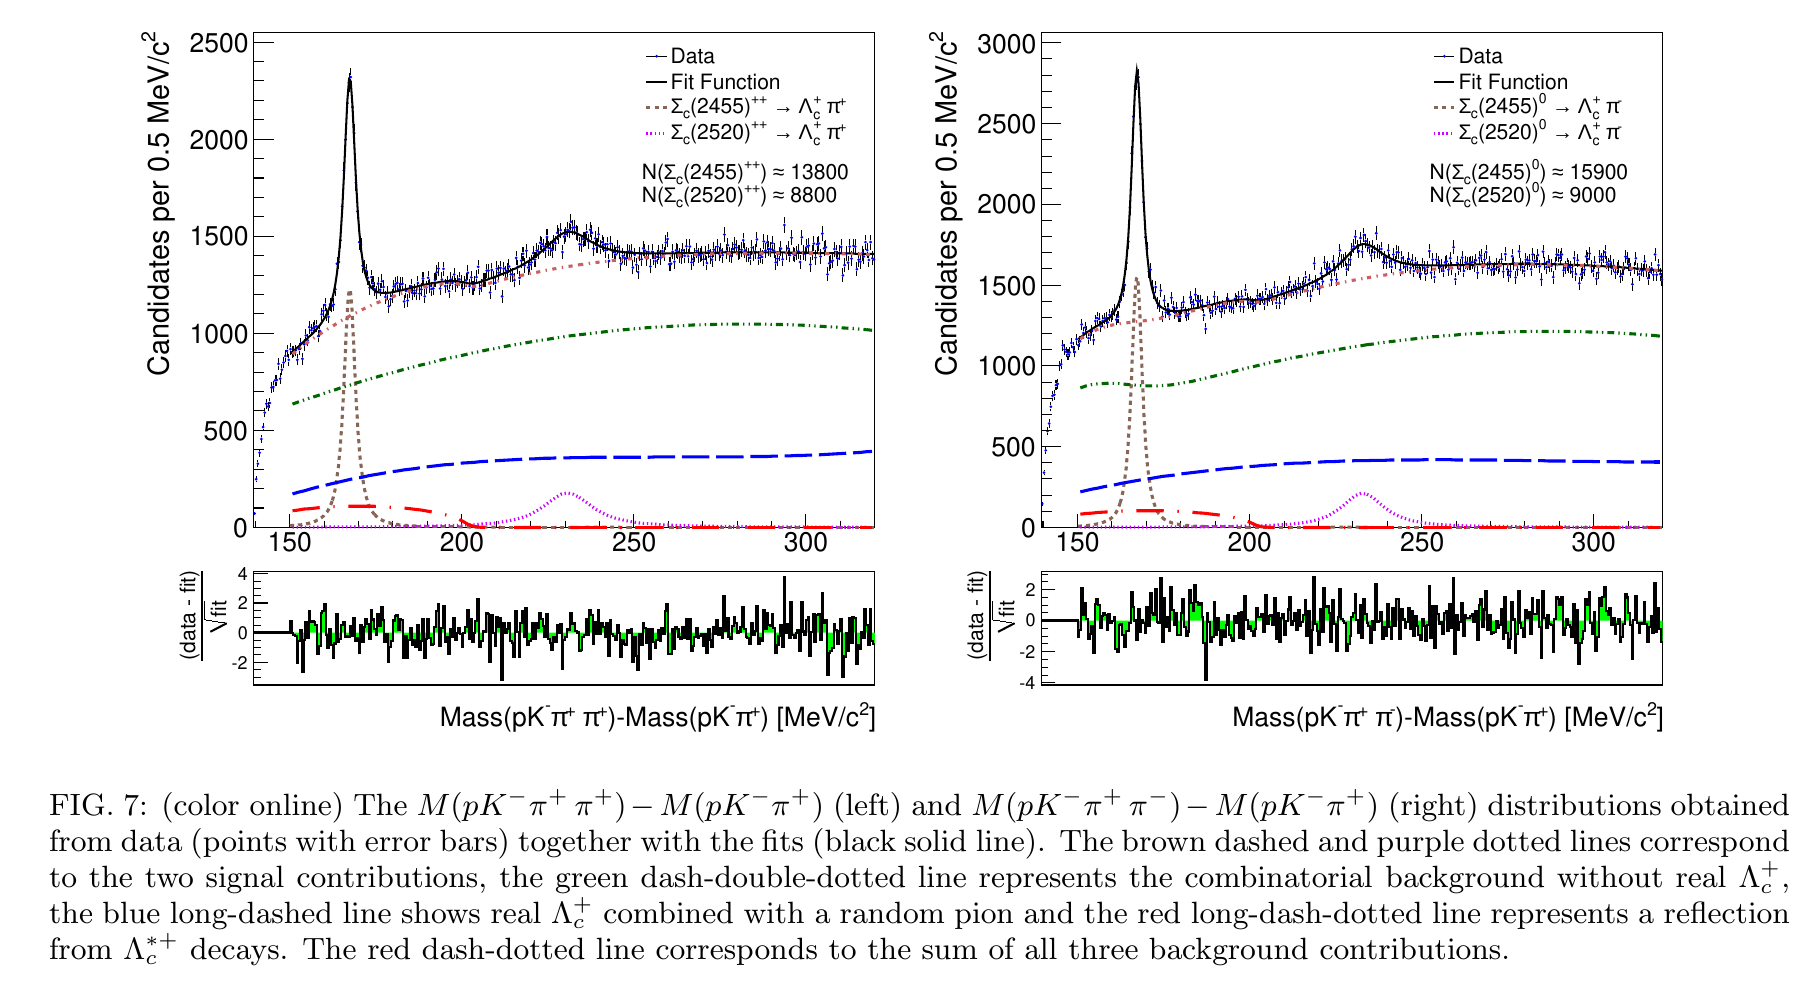
\includegraphics[width=\textwidth]{figures/001/fit-Scstar}

  % To fit the Lcpi spectra a model with three backgrounds and two 
  % signals was used. The three backgrounds represent completely random 
  % track combinations (green), combinations of real Lc with random pi 
  % (blue) and decays of Lc2625 resonance. Backgrounds are modeled by 
  % polynomials and signals by BW. The threshold is avoided to simplify 
  % the model.
\end{frame}%}}}

\begin{frame}[label=fit-Lc*]%{{{
  \frametitle{Model and approximation of $\Lambda_c^+\pi^+\pi^-$ spectrum}
  %\centering
  \parbox[w]{.48\textwidth}{
    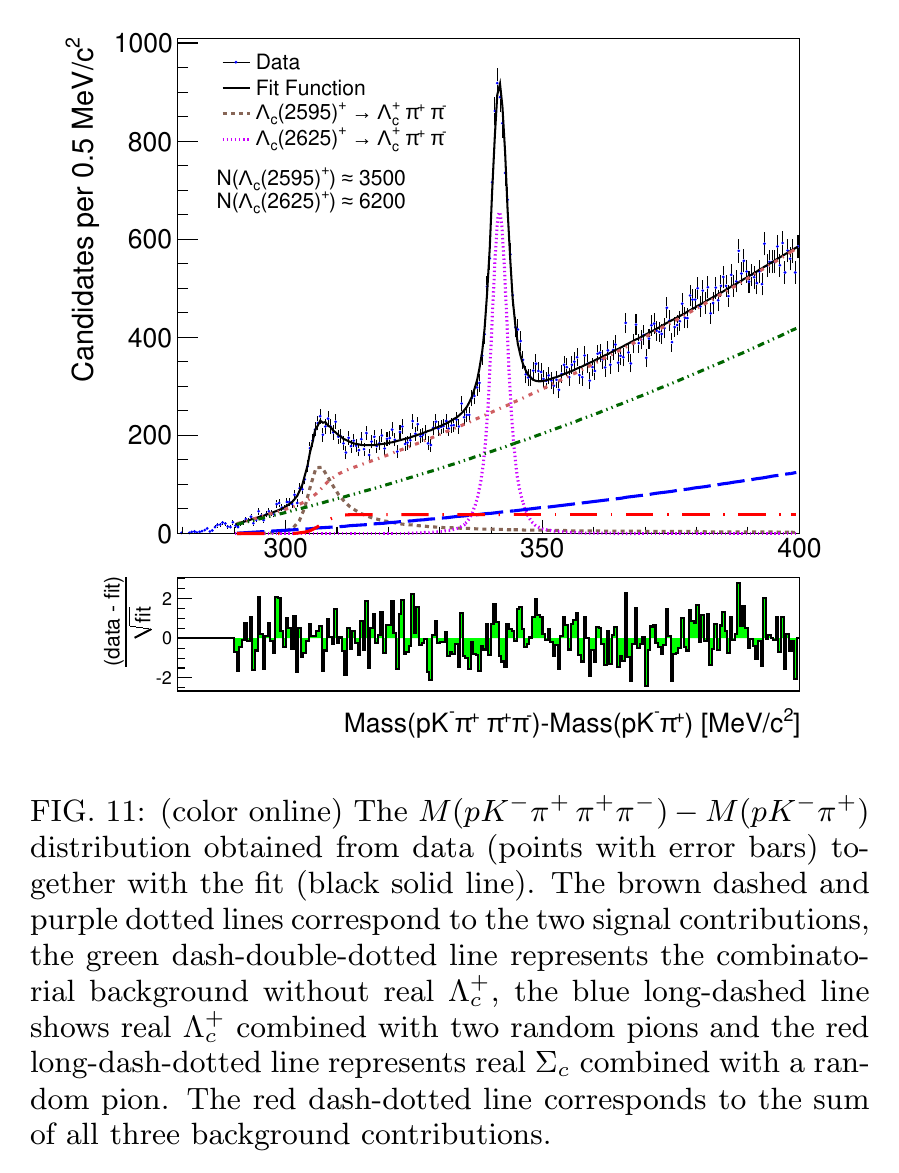
\includegraphics[width=.48\textwidth]{figures/001/fit-Lcstar}
  } \parbox[w]{.48\textwidth}{
    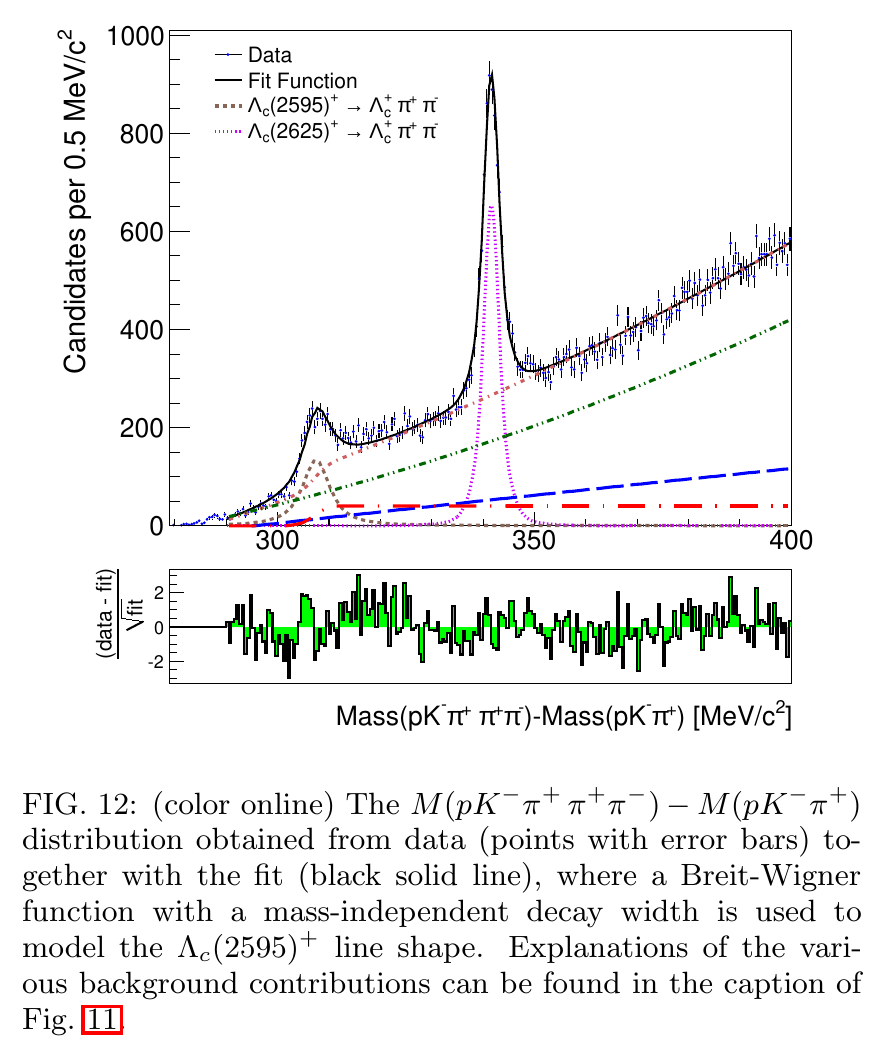
\includegraphics[width=.48\textwidth]{figures/001/fit-Lcstar-simple2595}
  }

  % An analogous model with 3 bkg and 2 sig is used for the Lcpipi 
  % spectrum. The third bkg here comes from combinations of real Sc with 
  % random pi. So there is cross-feed between the spectra. A major 
  % difference here is that Lc2595 cannot be described by a simple 
  % symmetric BW. Because of the extreme closeness of Lc2595 mass to Sc 
  % pi threshold, a very complex model with mass-dependent natural width 
  % is necessary.
\end{frame}%}}}

\begin{frame}[label=syst]%{{{
  \frametitle{Systematic uncertainties}
  \centering
  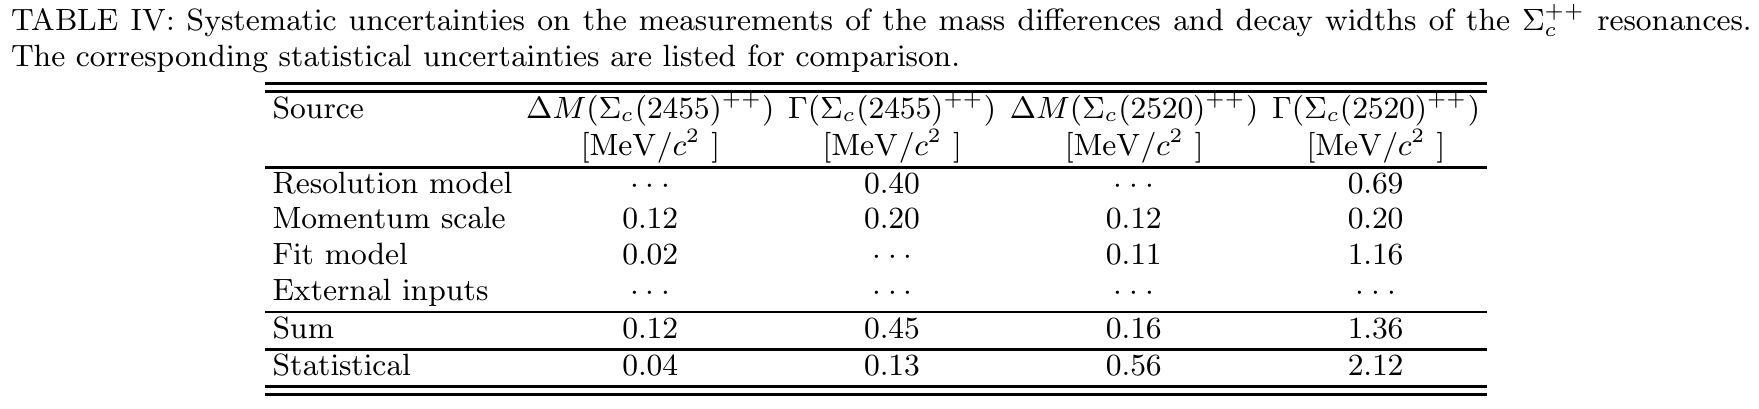
\includegraphics[width=.95\textwidth]{figures/001/syst-Scpp}
  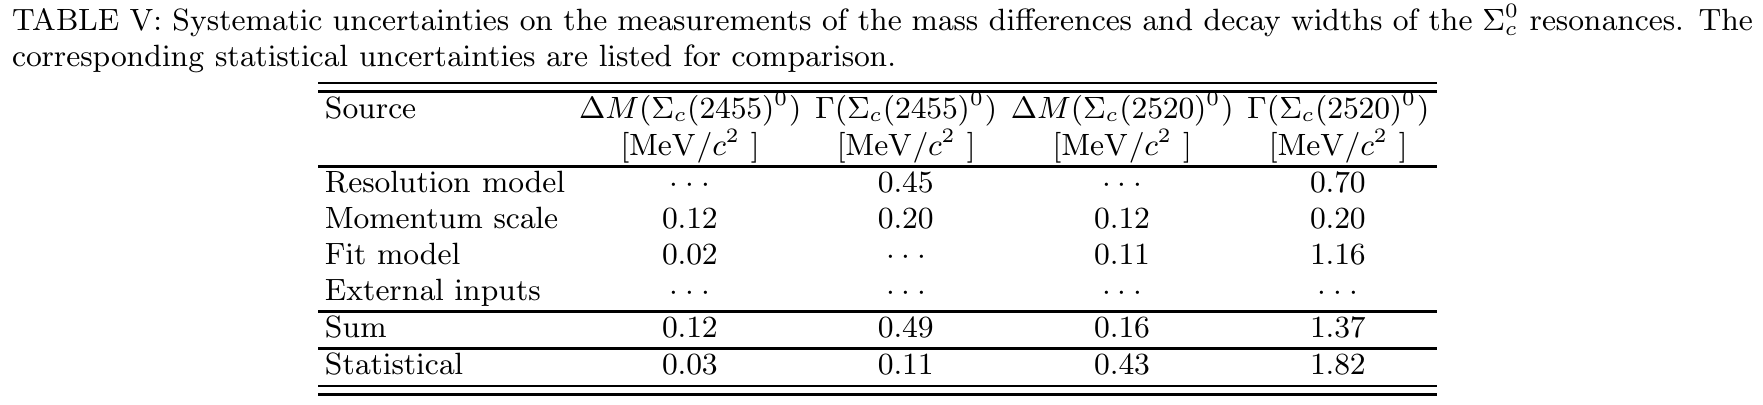
\includegraphics[width=.95\textwidth]{figures/001/syst-Scz}
  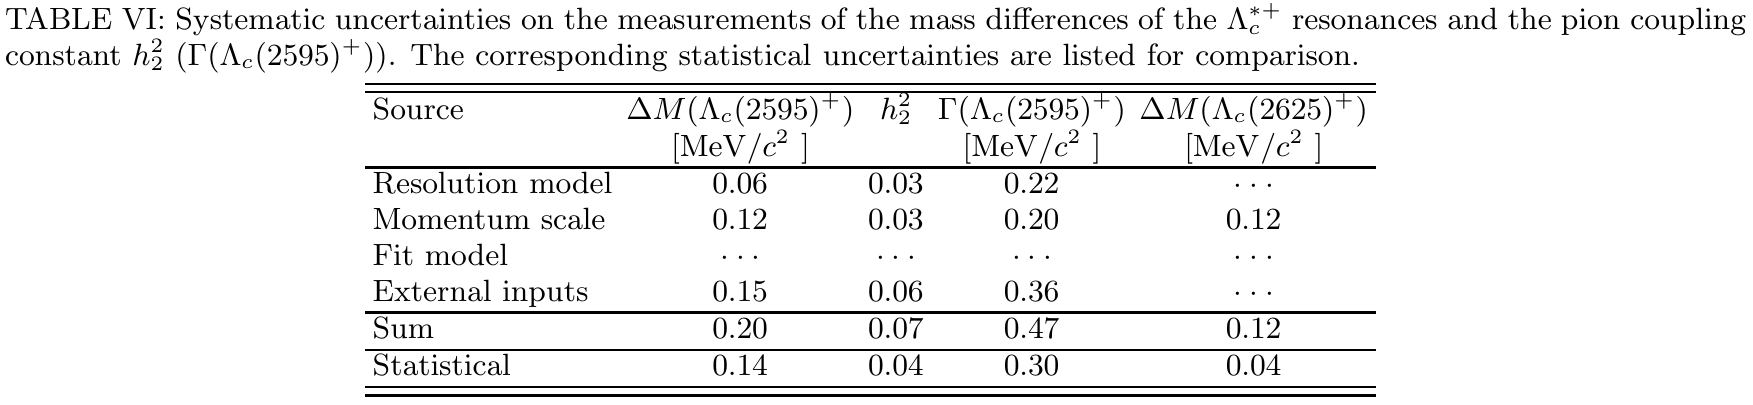
\includegraphics[width=.95\textwidth]{figures/001/syst-Lc}

  % So resonance parameters are measured from the three fits. The next 
  % step would naturally be to estimate syst uncertainties, which CDF 
  % obviously did. The following sources are considered.
\end{frame}%}}}

\begin{frame}[label=results]%{{{
  \frametitle{Results}
  \centering
  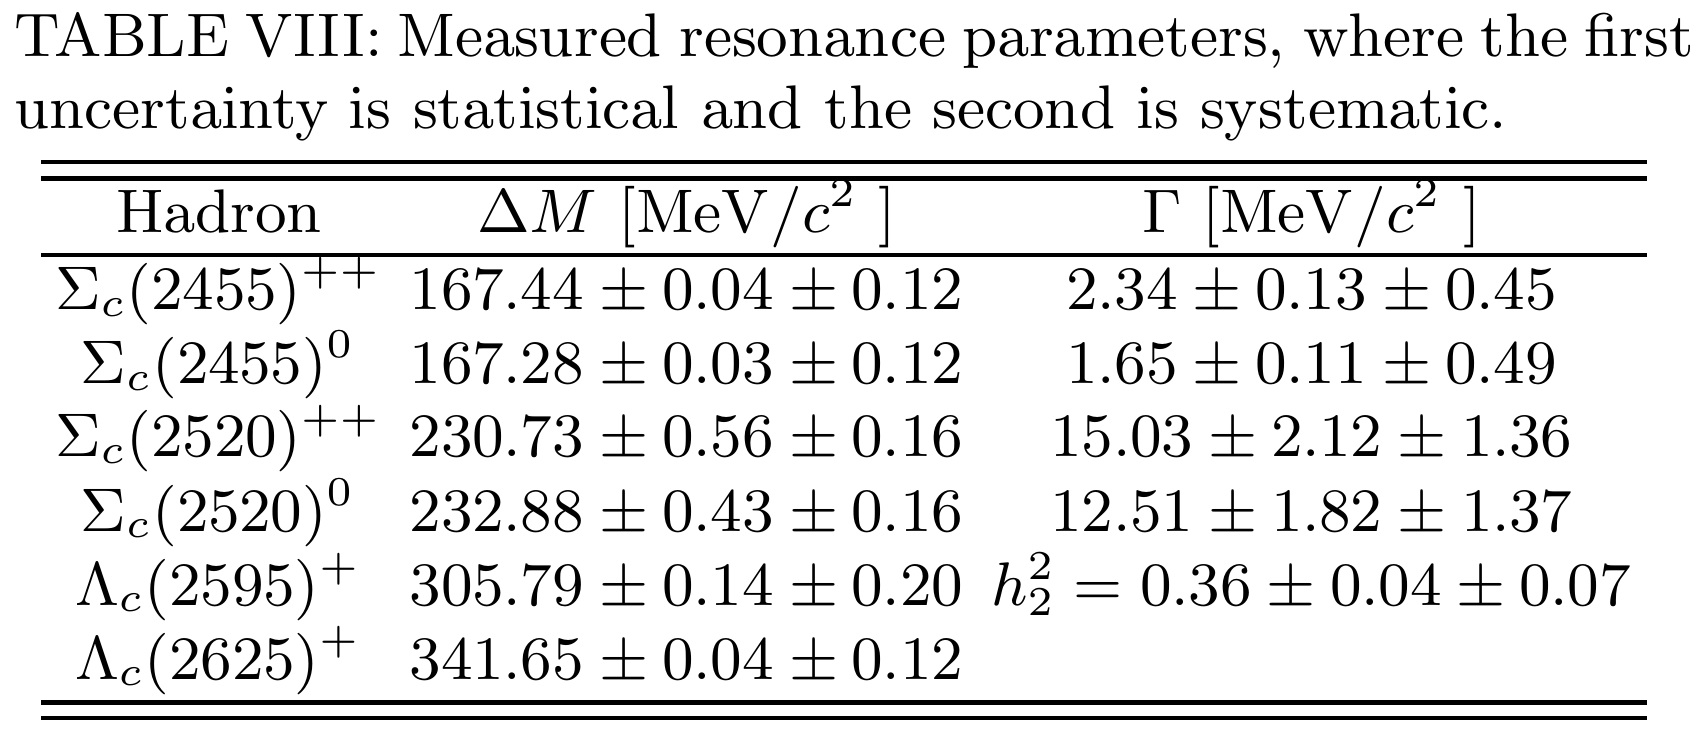
\includegraphics[width=.9\textwidth]{figures/001/results}
  $$ \Gamma(\Lambda_c(2595)^+) = 2.59 \pm 0.30 \pm 0.47 \text{\textrm{ MeV}} $$
\end{frame}%}}}

\end{document}


Vocabulary

Hadron
heavy quark
quantum chromodynamics
coupling constant
momentum
decay widths
framework (of a theory)
perturbative QCD
relativistic
lattice QCD
mesons
quantum electrodynamics
baryons
mass spectrum
splittings (masses of Sc isotriplets)
heavy flavor
sophisticated
proximity
charge-conjugate
intermediate
orbital excitations
ground state
cross-feed
collisions
detector
final state tracks
sum rules
bag model
tracking system
axial magnetic field
silicon microstrip detector
beam-pipe
plane
transverse
vertex
approximately
longitudinal
drift chamber
lokelihood
time-of-flight system
ionization
event selection
azimuthal
displaced
reconstruction
oppositely charged
simulated events
estimate
integrated (luminosity)
luminosity
accumulated
resonance structure
hypothesis
scattering
energy loss
kinematic
charge
neural network
Gaussian
linear
probability density function
input quantities (MVA variables)
uncertainty
neural network training
weight
resonant substructure
classify
randomly
complementary subsample
a posteriori
bias
statistical fluctuations
artificial excess (MVA bias)
yields
nominal (mass of a resonance -- expected)
neutral and doubly-charged states
proper decay time
kinematic fit
binned maximum likelihood fits
likelihood function
parameterized
mean zero (for resolution model)
scaling factor
resolution
second-order polynomial
normalization
spectra
D0 decay products
theoretical considerations
approximation
threshold
dominantly
natural width
nonresonant
Dalitz plot
projection
dependence
amounts (to something)
denominator
numerator
saturate
partial widths
S-wave decay
D-wave contribution
Gaussian constrained
float in the fit

SYSTEMATIC UNCERTAINTIES
momentum scale of the detector
add up the contributions from all sources in quadrature.
instantaneous luminosity
disentangle
negligible effect
magnetic field 
Gaussian error propagation.
internal consistency of the fit
analytic function
ensemble of statistical trials
signal to background ratio
unbiased.
absorb the tails of the relatively broad signal structure
rest frame
standard deviation 
Bayesian approach
credibility level 
excited charmed baryons
resonance parameters
hadron collider
